\documentclass[10pt,a4paper]{article}

\usepackage[margin=1.05in]{geometry}
\usepackage{setspace,amsmath,amssymb,amsthm}
\usepackage{graphicx,enumitem,titlesec,fancyhdr,microtype}
\usepackage{hyperref}
\graphicspath{{../../drawings/pass2/}}
\hypersetup{colorlinks=true,linkcolor=black,urlcolor=black,citecolor=black}

\titleformat{\section}{\normalsize\bfseries}{}{0em}{}
\titlespacing*{\section}{0pt}{1.35em}{0.5em}

\theoremstyle{plain}
\newtheorem{proposition}{Proposition}
\theoremstyle{definition}
\newtheorem{definition}{Definition}
\theoremstyle{remark}
\newtheorem{observation}{Observation}

\setstretch{1.14}
\pagestyle{fancy}
\fancyhf{}
\fancyhead[L]{\small\itshape Elements of Position}
\fancyhead[R]{\small\itshape V.\ Already There}
\fancyfoot[C]{\small\thepage}
\renewcommand{\headrulewidth}{0pt}

\begin{document}

\begin{center}
\vspace*{1.8em}
{\large Elements of Position}\\[1.4em]
{\LARGE\bfseries V.\ Already There}\\[0.4em]
{\small Furniture that was waiting inside the pair}\\[1.4em]
{\normalsize Justin Erholtz}\\[0.3em]
{\small 24 September 2026}
\end{center}

\vspace{1.0em}

\begin{center}
{\large The pieces were old. The wiring had not been named.}
\end{center}

\vspace{0.8em}

\noindent
\textit{A note.}
This part is not a new construction.
It asks further questions of objects Parts~I--IV already finished.
Cassini's closed form for docking, once drafted here, now lives in Part~IV, where the docking itself was named.
Plates G1 and SB1 read the recorded crossings table and the pair.

\tableofcontents

\section{The wedge residual is digamma}

Grows out of: the constant \(\gamma/2-1/4\) first seen by comparing the discrete sum of \(\tau\) to its integral.

\begin{proposition}
\(H_N=\psi(N+1)+\gamma\).
The trapezoidal residual of the \(1/(2n)\) term of \(\tau\) is the Stirling series for \(\psi\).
\end{proposition}

At \(N=127\) on the recorded run, discrete sum minus trapezoid equals \(0.038605\), against \(\gamma/2-1/4=0.0386078\ldots\).

The Bernoulli ladder at fixed \(N\) descends and then diverges.
That divergence is vacuum and trace inside eighteenth-century analysis.
It is not a license to treat an asymptotic series as a last tick.

A first misreading of the growing gap between a running total of \(\tau\) and the bare integral blamed floating-point loss.
A Kahan-compensated total disagrees from the integral by the same amount.
Nothing was lost in the addition.
The missing term was the Euler--Maclaurin correction named above.

\section{The gap word}

Grows out of: Part~II, sheet SCH1; S\'os; \'Swierczkowski.

On the \(24\)~September run: \(102\) long gaps, \(25\) short, word of twenty-five copies of \texttt{LLLLS} and a tail \texttt{LL}.

\[
1-\{\lambda\}=0.201578812235,\qquad
1-\{\lambda\}=[0;4,1,24,\ldots].
\]

Convergents: \(1/4\), \(1/5\), \(25/124\), \(26/129\).
The five is the denominator of the first simple approximation to the short frequency.
The \(124\) and \(129\) are the first defects.

A letter-exact match to a Sturmian word additionally requires a phase in a narrow interval.
The count-level split does not.


\begin{figure}[htbp]
\centering
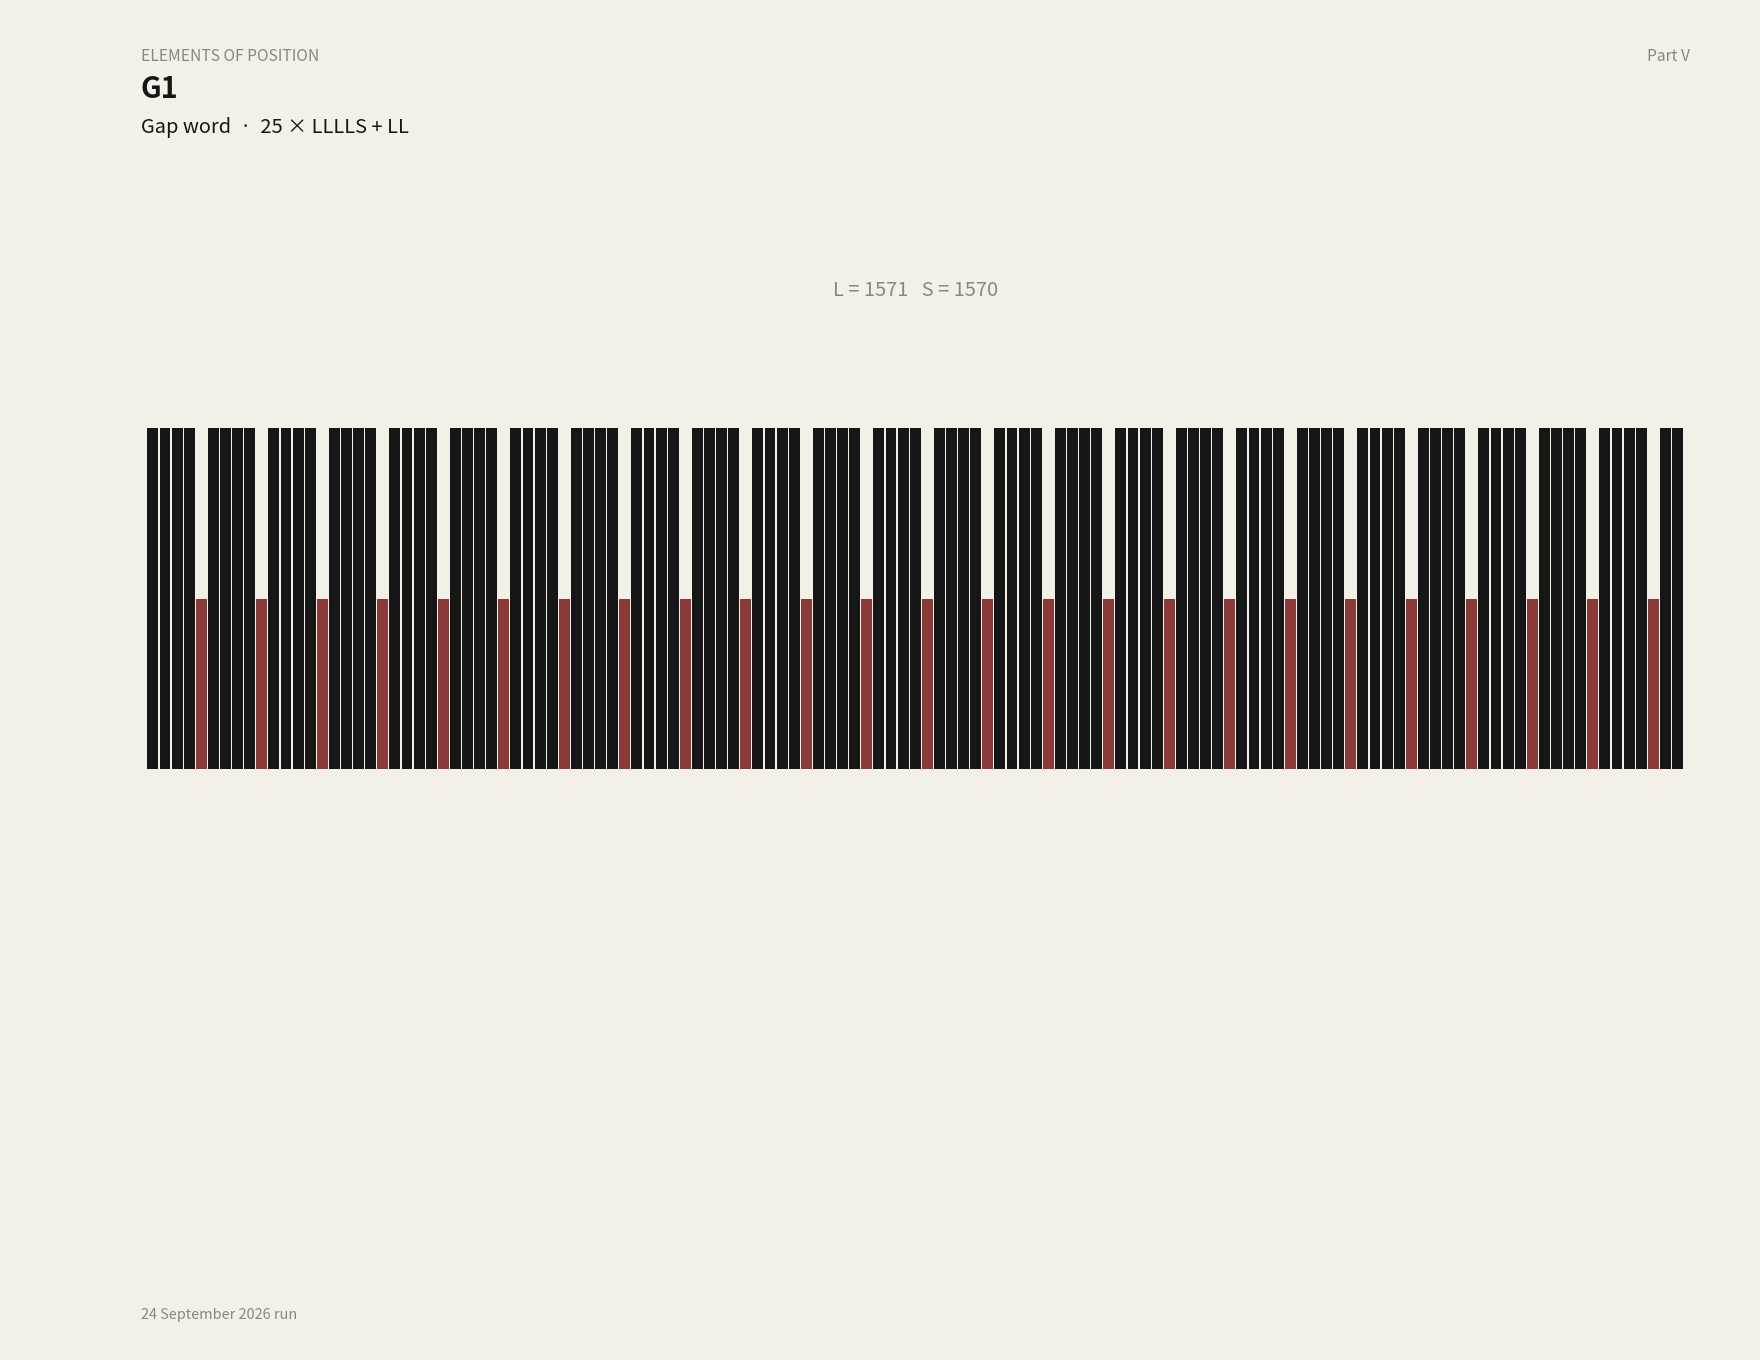
\includegraphics[width=0.92\textwidth]{G1_word.png}
\caption{Sheet G1. The recorded word: twenty-five copies of LLLLS, tail LL.}
\end{figure}

\section{One tree underneath both processes}

The Stern--Brocot right spine is \(1,2,3,\ldots\).
The left spine is \(1,1/2,1/3,\ldots\).
Those are the pair of Part~I.
Inversion is the tree's reflection on its boundary, not an operation imported from outside it.


\begin{figure}[htbp]
\centering
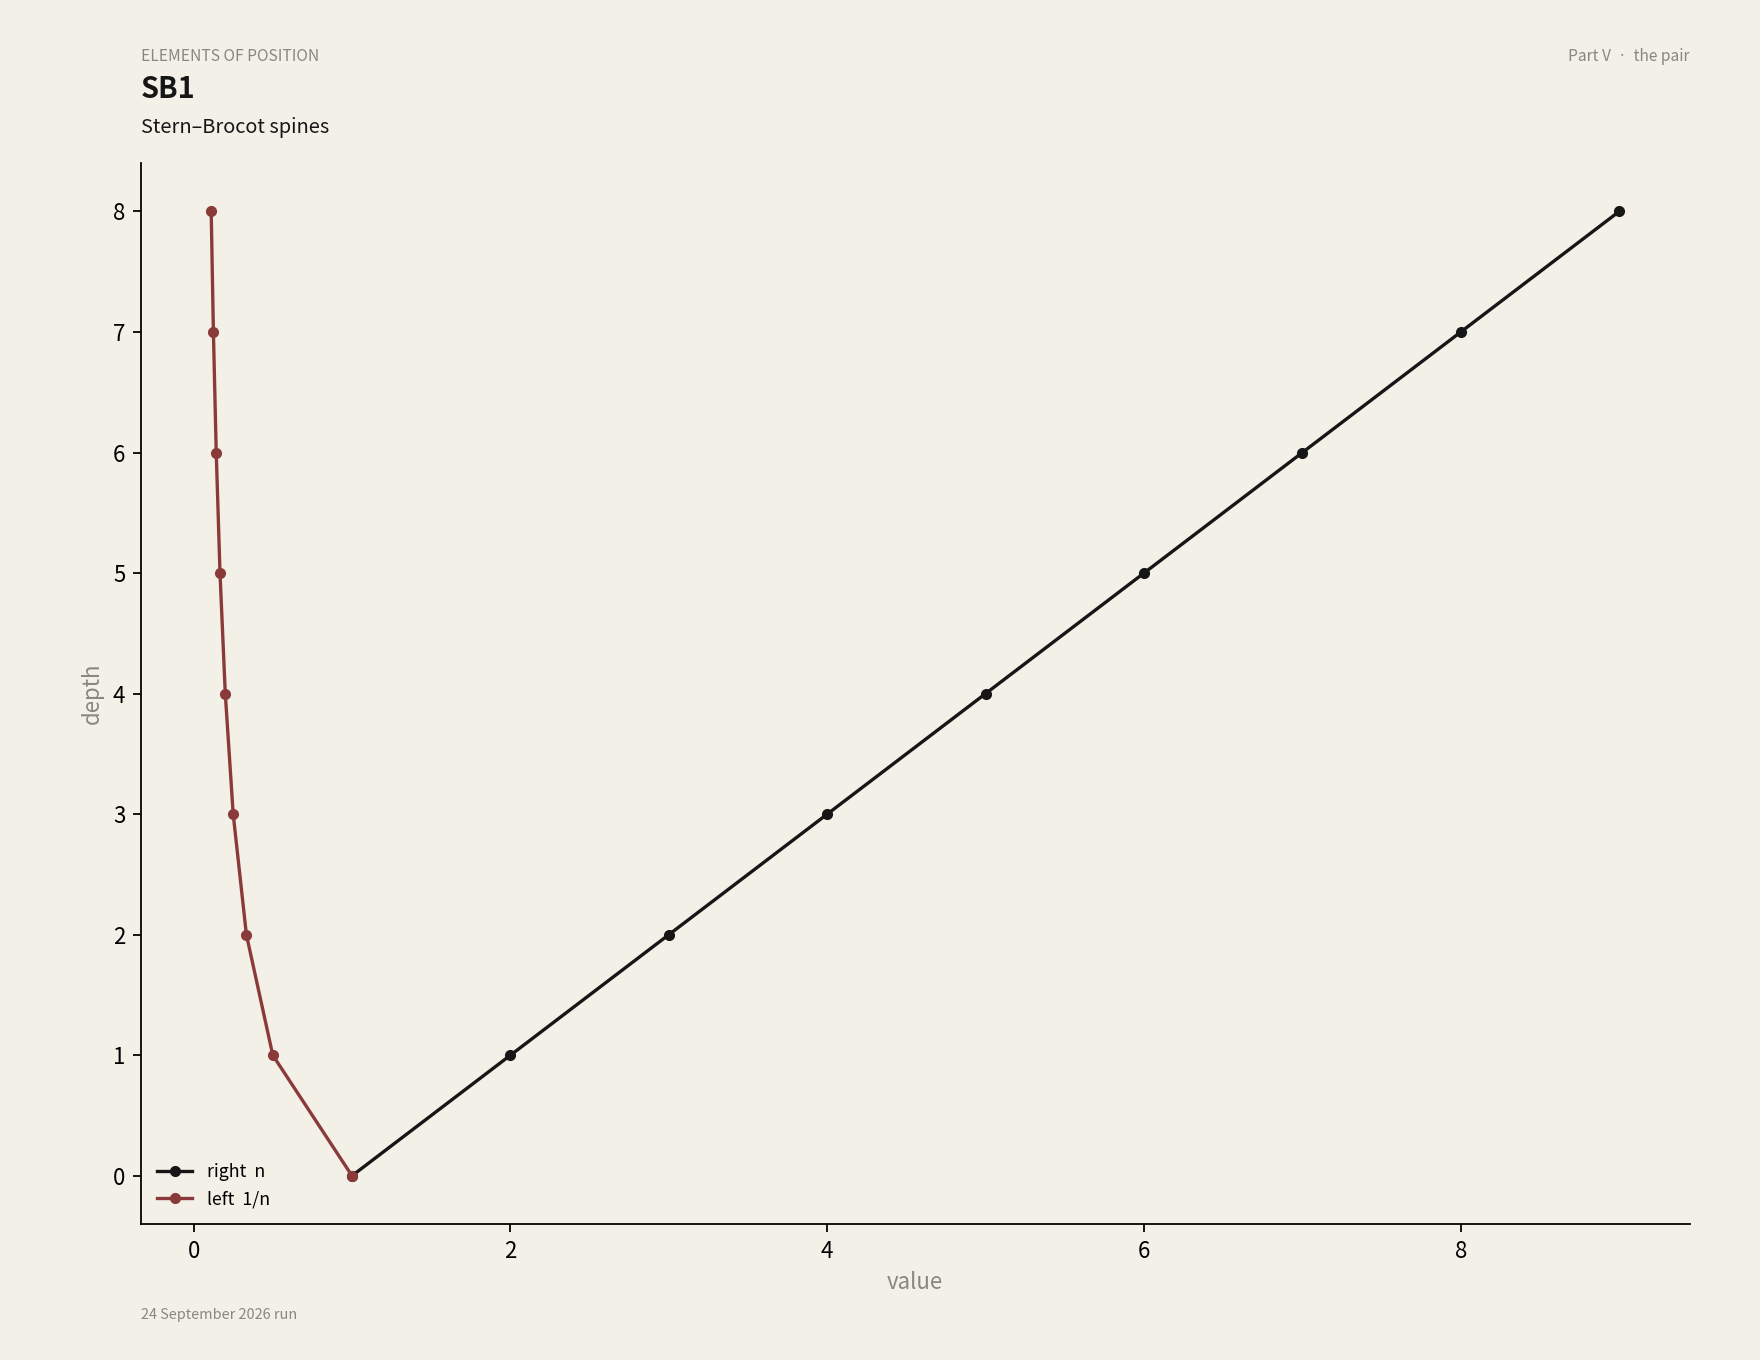
\includegraphics[width=0.92\textwidth]{SB1_spines.png}
\caption{Sheet SB1. Right spine $n$, left spine $1/n$.}
\end{figure}

The alternating path produces consecutive Fibonacci ratios.
Unimodularity holds on every path: consecutive nodes satisfy \(p_k q_{k-1}-p_{k-1}q_k=\pm 1\).
Cassini is the periodic case; its docking consequence is Part~IV.

\section{What did not arrive}

HM and QM of \((n,1/n)\) collapse onto AM.
They are not carried forward.

No numeric relation between \(\gamma\) and \(\varphi\) was found, and none was manufactured.

\section{What stands}

Forced:
the digamma identification of the wedge residual;
the gap word's counts and the continued fraction of \(1-\{\lambda\}\), checked on the live CSV;
the Stern--Brocot spines as the pair.

Not granted:
Cassini as a result of this part (it stands in Part~IV);
a letter-exact Sturmian match without a named phase.

Where is \(1\)?
Every result above was reached by standing at the lock and asking what else was already true about the two numbers on either side of it.

\end{document}
